\documentclass{article}
\usepackage{graphicx}
\usepackage{listings}
\usepackage{xcolor}
\usepackage{amsmath}
\usepackage{geometry}

\geometry{margin=1in}

\lstset{
  language=C++,
  basicstyle=\ttfamily\small,
  keywordstyle=\color{blue},
  commentstyle=\color{green!60!black},
  stringstyle=\color{red},
  breaklines=true,
  breakatwhitespace=true,
  showstringspaces=false,
  frame=single,
  numbers=left,
  numberstyle=\tiny\color{gray},
  stepnumber=1,
  tabsize=2
}

\title{Building an Arduino Calculator with Breadboard and Push Buttons}
\author{Niketh Achanta - EE24BTECH11047}
\date{}

\begin{document}

\maketitle

\section{Introduction}

This report details the process of building a functional calculator using an Arduino microcontroller, a breadboard, push buttons, and an LCD display. The calculator can perform basic arithmetic operations (addition, subtraction, multiplication, and division) as well as trigonometric functions (sine, cosine, tangent, and their inverse functions). This project demonstrates fundamental concepts in embedded systems programming, user interface design, and mathematical computation.

\section{Materials Required}

\begin{itemize}
    \item Arduino board (UNO)
    \item Breadboard
    \item 16x2 LCD display
    \item Push buttons (at least 14)
    \item Jumper wires
    \item Potentiometer (For LCD brightness contrast)
\end{itemize}

\section{Circuit Design}

The calculator circuit consists of three main components:

\subsection{LCD Display}
\begin{figure}[h]
    \centering
    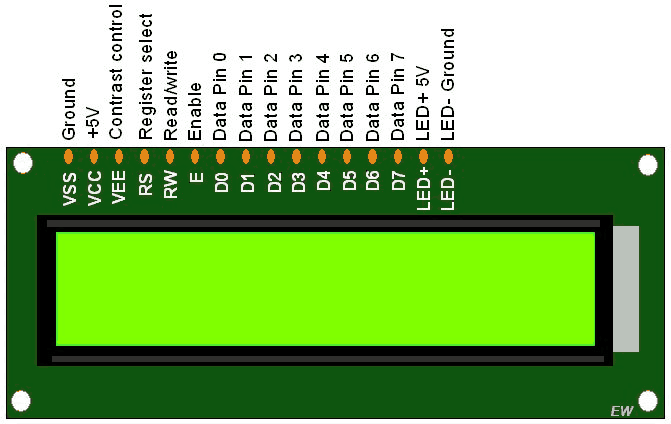
\includegraphics[width=0.5\textwidth]{figs\LCD.png}
    \caption{LCD Display Pinout}
\end{figure}
The 16x2 LCD display is connected to the Arduino in 4-bit mode to save pins. The connections are as follows:

\begin{itemize}
    \item RS (Register Select) pin connected to Arduino pin 1 (PD1)
    \item E (Enable) pin connected to Arduino pin 0 (PD0)
    \item D4 connected to Arduino pin 5 (PD5)
    \item D5 connected to Arduino pin 4 (PD4)
    \item D6 connected to Arduino pin 3 (PD3)
    \item D7 connected to Arduino pin 2 (PD2)
\end{itemize}

\subsection{Push Buttons}

The calculator uses multiple push buttons for input:
\begin{itemize}
    \item Numeric buttons (0-9) connected to Arduino pins 13 (PB5) through 8 (PB0) and pins 7 (PD7), 6 (PD6), A0 (PC0), and A1 (PC1)
    \item Operator button (cycles through +, -, *, /) connected to Arduino pin A2 (PC2)
    \item Trigonometric function button (cycles through sin, cos, tan, asin, acos, atan) connected to Arduino pin A3 (PC3)
    \item Decimal point button connected to Arduino pin A4 (PC4)
    \item Enter/equals button connected to Arduino pin A5 (PC5)
\end{itemize}



\section{Wiring}

The wiring should be done as follows:
\begin{enumerate}
    \item Connect the LCD pins as specified in the LCD Display section
    \item For each button:
        \begin{itemize}
            \item Connect one terminal to the corresponding Arduino pin
            \item Connect the other terminal to ground
        \end{itemize}
    \item Connect the Arduino's 5V and GND pins to the breadboard's power rails
\end{enumerate}

\section{Code Explanation}

This section provides a detailed explanation of the scientific calculator implementation for an AVR microcontroller.

\subsection{Overview}
The code implements a scientific calculator on an AVR microcontroller with an LCD display and a button interface. It supports basic arithmetic operations and trigonometric functions. The calculator allows users to input numeric values, select operations, and compute results.

\subsection{Hardware Configuration}
\begin{itemize}
    \item \textbf{LCD Interface:} Connected to PORTB with RS pin on PB0 and EN pin on PB1
    \item \textbf{Button Interface:} 
    \begin{itemize}
        \item Numeric buttons (0-7): Connected to PORTD pins PD0-PD7
        \item Numeric buttons (8-9): Connected to PORTC pins PC0-PC1
        \item Decimal point button: Connected to PC2
        \item Operation selection button: Connected to PC3
        \item Trigonometric function button: Connected to PC4
        \item Enter button: Connected to PC5
    \end{itemize}
\end{itemize}

\subsection{Key Components}

\subsubsection{LCD Control Functions}
\begin{itemize}
    \item \texttt{lcd\_init()}: Initializes the LCD in 4-bit mode
    \item \texttt{lcd\_cmd()}: Sends command instructions to the LCD
    \item \texttt{lcd\_data()}: Sends character data to display on the LCD
    \item \texttt{lcd\_print()}: Outputs a string to the LCD
\end{itemize}

\subsubsection{Button Handling}
\begin{itemize}
    \item \texttt{init\_buttons()}: Configures button pins as inputs with pull-up resistors
    \item \texttt{check\_button()}: Detects button presses with debouncing logic
\end{itemize}

\subsubsection{Expression Handling}
\begin{itemize}
    \item \texttt{append\_char()}: Adds a character to the expression buffer
    \item \texttt{update\_lcd()}: Refreshes the LCD with the current expression
    \item \texttt{append\_operator()}: Handles addition of arithmetic operators (+, -, *, /)
    \item \texttt{append\_trig\_function()}: Handles addition of trigonometric functions
    \item \texttt{process\_enter()}: Placeholder for expression evaluation
\end{itemize}

\subsection{Program Flow}
The main program follows this execution flow:
\begin{enumerate}
    \item Initialize the expression buffer, LCD, and button interface
    \item Display a welcome message prompting the user to enter an expression
    \item Enter the main loop that continuously monitors button presses:
    \begin{itemize}
        \item Decimal point button adds a decimal point to the current number
        \item Numeric buttons (0-9) append digits to the expression
        \item Operation button cycles through arithmetic operators
        \item Trigonometric button cycles through trig functions
        \item Enter button processes the expression (evaluation logic is a placeholder)
    \end{itemize}
\end{enumerate}

\subsection{Features and Behavior}
\begin{itemize}
    \item Automatically inserts a leading zero when adding a decimal point after an operator
    \item Prevents multiple decimal points within a single number
    \item Supports nesting of functions (e.g., sin(cos(x)))
    \item Clears the display when entering a new expression after a result
    \item Cycles through operators (+, -, *, /) and trigonometric functions (sin, cos, tan, asin, acos, atan)
\end{itemize}

\subsection{Implementation Considerations}
\begin{itemize}
    \item The code uses a fixed-size buffer (\texttt{MAX\_EXPR\_LENGTH = 32}) to store the expression
    \item Debouncing is implemented with delay functions
    \item The actual expression evaluation logic is not implemented in the current version
    \item Button state tracking prevents duplicate entries and ensures proper syntax
\end{itemize}
\section{Mathematical Implementation}

The calculator implements mathematical operations using a recursive descent parser in the \texttt{evaluate\_expression()} function. This approach allows it to handle complex expressions with nested parentheses and functions.

For trigonometric functions, the calculator converts between degrees and radians:
\begin{itemize}
    \item For direct trig functions (sin, cos, tan), it converts the input from degrees to radians using the formula $$ \text{radians} = \text{degrees} \times \pi / 180 $$
    \item For inverse trig functions (asin, acos, atan), it converts the output from radians to degrees using $$ \text{degrees} = \text{radians} \times 180 / \pi $$
\end{itemize}

The calculator also handles special cases like division by zero, which returns NaN (Not a Number).

\section{Conclusion}

This Arduino calculator project demonstrates how to build a functional calculator using basic electronic components and programming techniques. The implementation includes:

\begin{itemize}
    \item Hardware interfacing with an LCD display and push buttons
    \item User input processing and display
    \item Mathematical expression parsing and evaluation
    \item Error handling for cases like division by zero
\end{itemize}

The project can be extended in several ways, such as adding more mathematical functions, improving the user interface, or adding memory functions.
\section{References}
\begin{enumerate}
    \item Code By MBS Aravind
    \item AI suggestions for connections and other hardware analysis
    \item Stock pictures for pinout diagrams
\end{enumerate}
\end{document}
